\chapter[SCP-043 披头不四]{
    SCP-043 The Beatle\\
    SCP-043 披头不四
}

\label{chap:SCP-043}

\begin{figure}[H]
    \centering
    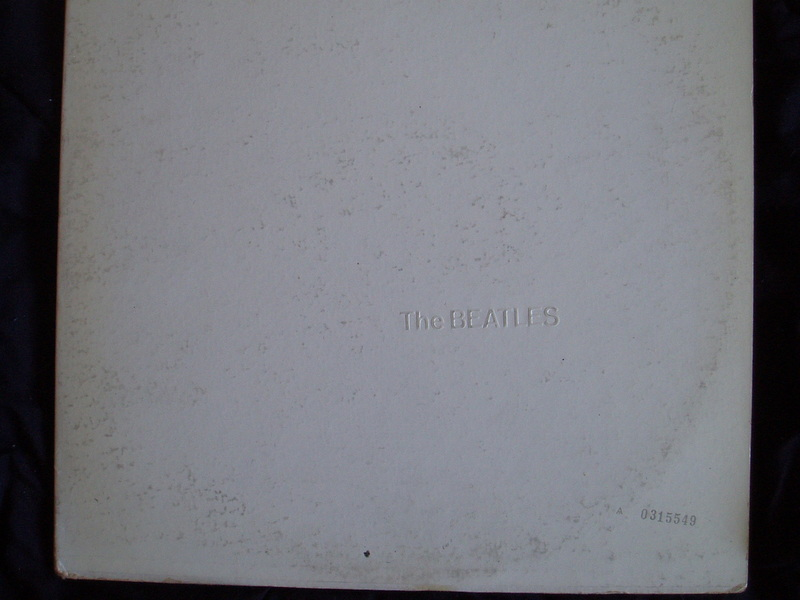
\includegraphics[width=0.5\linewidth]{images/SCP.043.jpg}
    \caption*{SCP-043,在其封套内。}
\end{figure}

\bb{项目编号:}SCP-043

\bb{项目等级:}Safe

\bb{特殊收容措施:}SCP-043不需要特殊收容,但不推荐将SCP-043用于实验以外的用途。一个唱机应随时放置于同一个房间以用于进行实验。

\bb{描述:}SCP-043外观是披头士乐队的唱片“The White Album”的一张塑料复刻版。但是,在最近的检查中发现这张唱片上没有沟槽。可无论唱针的起始位置在哪,唱片仍能从头到尾播放。

当播放到第29首歌曲的时候,唱片不会播放曲目“Revolution 9”,而是停止了旋转,且能听到微弱的呼吸声。有时发出呼吸声的实体会用一把男性的声音说话。该实体会回答对其的提问,且在音乐界、乐理、许多乐队和艺术家的八卦琐事方面显露出渊博的百科全书式的知识。然而,该实体拒绝回答关于披头士乐队或它自身的个人细节方面的问题。

在唱片的外包装里,找到了一小张手写的纸条,上面写着:

\begin{scpbox}

\ii{限量版:1\slash 1}

\ii{谢啦, John!}

\ii{xxx}

\end{scpbox}
